\onlyinsubfile{\setcounter{section}{3}}
\section{Results}\notinsubfile{\label{sec:results}}
%\setcounter{page}{0}\pagenumbering{arabic}

\subsection{Income and trust}

\par First, I wanted to see if the \say{hump-shape} relationship between trust and income found by \cite{jbpglg2016} was present in the HRS data. To do this I used the available income data from the 2020 wave with the trust measures from the same year.


\begin{table}[htbp]\centering
\def\sym#1{\ifmmode^{#1}\else\(^{#1}\)\fi}
\caption{Log Income (2020) on Trust rv557}
\begin{tabular}{l*{4}{c}}
\toprule
          &\multicolumn{1}{c}{(1)}&\multicolumn{1}{c}{(2)}&\multicolumn{1}{c}{(3)}&\multicolumn{1}{c}{(4)}\\
          &\multicolumn{1}{c}{log Lab}&\multicolumn{1}{c}{log Tot}&\multicolumn{1}{c}{log Lab}&\multicolumn{1}{c}{log Tot}\\
& \multicolumn{2}{c}{No controls} & \multicolumn{2}{c}{With controls} \\\\ \cmidrule(lr){2-3}\cmidrule(lr){4-5}
Trust     &    0.282\sym{***}&    0.318\sym{***}&    0.153\sym{***}&    0.133\sym{**} \\
          &  (0.053)         &  (0.057)         &  (0.053)         &  (0.053)         \\
Trust$^{2}$&   -0.022\sym{***}&   -0.025\sym{***}&   -0.013\sym{***}&   -0.011\sym{***}\\
          &  (0.004)         &  (0.005)         &  (0.004)         &  (0.004)         \\
Age       &                  &                  &    0.048         &    0.123\sym{**} \\
          &                  &                  &  (0.045)         &  (0.052)         \\
Age$^{2}$ &                  &                  &   -0.000         &   -0.001\sym{**} \\
          &                  &                  &  (0.000)         &  (0.000)         \\
Years of education&                  &                  &    0.073\sym{***}&    0.098\sym{***}\\
          &                  &                  &  (0.011)         &  (0.012)         \\
In labor force&                  &                  &    0.667\sym{***}&    0.849\sym{***}\\
          &                  &                  &  (0.082)         &  (0.089)         \\
Married   &                  &                  &    0.098         &    0.243\sym{***}\\
          &                  &                  &  (0.061)         &  (0.066)         \\
Born in U.S.&                  &                  &    0.168\sym{*}  &    0.139         \\
          &                  &                  &  (0.099)         &  (0.115)         \\
\_cons    &    9.348\sym{***}&    9.447\sym{***}&    6.453\sym{***}&    3.422\sym{*}  \\
          &  (0.154)         &  (0.164)         &  (1.555)         &  (1.815)         \\
\midrule
Observations&  972.000         & 1023.000         &  963.000         & 1013.000         \\
Adj. R-squared&    0.038         &    0.034         &    0.193         &    0.221         \\
\bottomrule
\multicolumn{5}{l}{\footnotesize Standard errors in parentheses}\\
\multicolumn{5}{l}{\footnotesize Robust SEs in parentheses; Age entered quadratically when available.}\\
\multicolumn{5}{l}{\footnotesize Controls (when included): raedyrs, in labor force, married, born in U.S.}\\
\multicolumn{5}{l}{\footnotesize \sym{*} \(p<0.10\), \sym{**} \(p<0.05\), \sym{***} \(p<0.01\)}\\
\end{tabular}
\end{table}




\par As you can see, the effect does persist in this dataset. These estimates suggest that the level of trust which maxmizes predicted income is $6.4, 6.36, 5.88, 6.05$.

\par Since the HRS includes multiple measures of trust, I do a principal component analysis (PCA) on them and use that as the explanatory variable. The results are in the table below.


\begin{table}[htbp]\centering
\def\sym#1{\ifmmode^{#1}\else\(^{#1}\)\fi}
\caption{Income 2020 on Trust PC1 (raw and with controls)}
\begin{tabular}{l*{8}{c}}
\toprule
                &\multicolumn{1}{c}{(1)}&\multicolumn{1}{c}{(2)}&\multicolumn{1}{c}{(3)}&\multicolumn{1}{c}{(4)}&\multicolumn{1}{c}{(5)}&\multicolumn{1}{c}{(6)}&\multicolumn{1}{c}{(7)}&\multicolumn{1}{c}{(8)}\\
                &\multicolumn{1}{c}{Respondent labor income (sum of 6 components; missing if all missing)}&\multicolumn{1}{c}{Respondent total income (labor + hwicap + hwiother; missing if all missing)}&\multicolumn{1}{c}{log(resp\_lab\_inc)}&\multicolumn{1}{c}{log(resp\_tot\_inc)}&\multicolumn{1}{c}{Respondent labor income (sum of 6 components; missing if all missing)}&\multicolumn{1}{c}{Respondent total income (labor + hwicap + hwiother; missing if all missing)}&\multicolumn{1}{c}{log(resp\_lab\_inc)}&\multicolumn{1}{c}{log(resp\_tot\_inc)}\\
\midrule
Standardized values of trust\_pca1&   2049.7         &   2833.8         &   0.0404         &   0.0300         &   1967.8         &   2291.8         &   0.0498         &   0.0208         \\
                & (1599.5)         & (2525.1)         & (0.0371)         & (0.0413)         & (1515.9)         & (2399.4)         & (0.0343)         & (0.0358)         \\
\addlinespace
Standardized values of trust\_pca1 $\times$ Standardized values of trust\_pca1&  -2572.7\sym{**} &  -3767.7\sym{*}  &  -0.0973\sym{***}&   -0.102\sym{***}&   -260.7         &    199.1         &  -0.0492\sym{*}  &  -0.0445\sym{*}  \\
                & (1078.9)         & (2026.2)         & (0.0304)         & (0.0325)         &  (932.1)         & (1781.0)         & (0.0261)         & (0.0267)         \\
\addlinespace
r15agey\_b:w15 r age (years) at ivw begmon&                  &                  &                  &                  &    735.6         &   1621.7         &   0.0276         &    0.120\sym{**} \\
                &                  &                  &                  &                  & (1750.0)         & (2467.2)         & (0.0391)         & (0.0491)         \\
\addlinespace
r15agey\_b:w15 r age (years) at ivw begmon $\times$ r15agey\_b:w15 r age (years) at ivw begmon&                  &                  &                  &                  &   -4.646         &   -10.41         &-0.000177         &-0.000781\sym{**} \\
                &                  &                  &                  &                  &  (13.64)         &  (18.16)         &(0.000281)         &(0.000344)         \\
\addlinespace
raedyrs: r years of education&                  &                  &                  &                  &   4150.6\sym{***}&   7059.7\sym{***}&   0.0824\sym{***}&   0.0993\sym{***}\\
                &                  &                  &                  &                  &  (604.2)         &  (942.1)         & (0.0109)         & (0.0124)         \\
\addlinespace
r15inlbrf:w15 =1 if r is in the labor force&                  &                  &                  &                  &  28151.4\sym{***}&  38378.8\sym{***}&    0.611\sym{***}&    0.819\sym{***}\\
                &                  &                  &                  &                  & (3600.9)         & (5445.3)         & (0.0726)         & (0.0886)         \\
\addlinespace
Married (r15mstat: 1 or 2) vs not married (3-8)&                  &                  &                  &                  &   5352.2         &  21783.2\sym{***}&    0.113\sym{*}  &    0.269\sym{***}\\
                &                  &                  &                  &                  & (4014.1)         & (5622.4)         & (0.0623)         & (0.0694)         \\
\addlinespace
Born in US (1) vs not US (0)&                  &                  &                  &                  &   6015.9\sym{*}  &   4595.9         &    0.227\sym{**} &    0.193         \\
                &                  &                  &                  &                  & (3541.9)         & (6126.9)         &  (0.108)         &  (0.124)         \\
\addlinespace
Constant        &  41714.7\sym{***}&  61237.1\sym{***}&    10.24\sym{***}&    10.44\sym{***}& -63940.1         &-130419.9         &    7.531\sym{***}&    3.933\sym{**} \\
                & (2563.6)         & (4111.9)         & (0.0415)         & (0.0494)         &(54991.7)         &(84341.0)         &  (1.345)         &  (1.735)         \\
\midrule
Observations    &      970         &      970         &      892         &      938         &      959         &      959         &      883         &      928         \\
Adj. R-squared  &  0.00353         &  0.00263         &   0.0194         &   0.0130         &    0.106         &    0.110         &    0.205         &    0.220         \\
\bottomrule
\multicolumn{9}{l}{\footnotesize Standard errors in parentheses}\\
\multicolumn{9}{l}{\footnotesize Robust SEs in parentheses; age entered quadratically when available}\\
\multicolumn{9}{l}{\footnotesize Controls:  raedyrs r15inlbrf married\_2020 born\_us}\\
\multicolumn{9}{l}{\footnotesize PC1 variance prop =      .}\\
\multicolumn{9}{l}{\footnotesize \sym{*} \(p<0.10\), \sym{**} \(p<0.05\), \sym{***} \(p<0.01\)}\\
\end{tabular}
\end{table}



\par These results are less encouraging. 

\subsection{Returns and trust}

\par With the hump-shape relationship between log earnings and trust present in the HRS, I wanted to see if a similar relationship held for returns. I used the formula from \cite{Daminato2024}: $$ r_t = \frac{y^c_t + cg_t -y^d_t}{A_{t-1} + .5F_t}   $$ where $y^c_t$ interest income and dividends, capital gains $cg_t$ measured as the difference between reported stock across waves, $F_t$ net investment flows, $y^d_t$ payments on debt (in the RAND longitudinal file, the variables were mentioned are all in net terms so this variable was $0$), and $A_{t-1}$ total net wealth at beginning of previous period.

\par Since the survey is every two years, I annualized the returns using the expression $r_annual = (1 + R_period)^(1/2) - 1$. I also trimmed the returns at the top and botton by $5\%$ to deal with outliers. The returns from residential housing were especially large, so I computed returns with this asset class excluded as well. 

\par Here are the results of the regression with the general trust measure as the explanatory variable. As you can see, the results are significant for the untrimmed returns but lose significance when I trim them in most cases. The level of trust which maximizes predicted returns is  $5.07, 3, 5.6, 11, 5.07, 1.5, 4.9, 8.5$. Again, the PCA results are worse. 

\begin{landscape}

\begin{table}[htbp]\centering
\def\sym#1{\ifmmode^{#1}\else\(^{#1}\)\fi}
\caption{Returns 2022 on Trust rv557 (raw and with controls)}
\begin{tabular}{l*{8}{c}}
\toprule
                &\multicolumn{1}{c}{(1)}&\multicolumn{1}{c}{(2)}&\multicolumn{1}{c}{(3)}&\multicolumn{1}{c}{(4)}&\multicolumn{1}{c}{(5)}&\multicolumn{1}{c}{(6)}&\multicolumn{1}{c}{(7)}&\multicolumn{1}{c}{(8)}\\
                &\multicolumn{1}{c}{r\_annual\_2022}&\multicolumn{1}{c}{r\_annual\_trim\_2022}&\multicolumn{1}{c}{r\_annual\_excl\_2022}&\multicolumn{1}{c}{r\_annual\_excl\_trim\_2022}&\multicolumn{1}{c}{r\_annual\_2022}&\multicolumn{1}{c}{r\_annual\_trim\_2022}&\multicolumn{1}{c}{r\_annual\_excl\_2022}&\multicolumn{1}{c}{r\_annual\_excl\_trim\_2022}\\
\midrule
trust: people in general&   0.0706\sym{**} &   0.0121         &   0.0563\sym{***}&   0.0223\sym{***}&   0.0706\sym{**} &  0.00330         &   0.0488\sym{***}&   0.0172\sym{*}  \\
                & (0.0279)         & (0.0189)         & (0.0169)         &(0.00839)         & (0.0282)         & (0.0193)         & (0.0172)         &(0.00905)         \\
\addlinespace
trust: people in general $\times$ trust: people in general& -0.00707\sym{***}& -0.00155         & -0.00536\sym{***}& -0.00148\sym{*}  & -0.00660\sym{***}&-0.000826         & -0.00455\sym{***}&-0.000997         \\
                &(0.00260)         &(0.00156)         &(0.00173)         &(0.000806)         &(0.00255)         &(0.00157)         &(0.00170)         &(0.000835)         \\
\addlinespace
r15agey\_b:w15 r age (years) at ivw begmon&                  &                  &                  &                  &  -0.0717\sym{**} &  0.00657         &  -0.0242         & -0.00844         \\
                &                  &                  &                  &                  & (0.0281)         & (0.0143)         & (0.0253)         &(0.00879)         \\
\addlinespace
r15agey\_b:w15 r age (years) at ivw begmon $\times$ r15agey\_b:w15 r age (years) at ivw begmon&                  &                  &                  &                  & 0.000482\sym{**} &-0.0000555         & 0.000154         &0.0000574         \\
                &                  &                  &                  &                  &(0.000201)         &(0.000102)         &(0.000181)         &(0.0000631)         \\
\addlinespace
raedyrs: r years of education&                  &                  &                  &                  &  0.00314         &  0.00460         &  0.00264         &  0.00165         \\
                &                  &                  &                  &                  &(0.00603)         &(0.00324)         &(0.00413)         &(0.00187)         \\
\addlinespace
r15inlbrf:w15 =1 if r is in the labor force&                  &                  &                  &                  &   0.0560         &   0.0470\sym{**} &   0.0600\sym{*}  &   0.0306\sym{**} \\
                &                  &                  &                  &                  & (0.0417)         & (0.0230)         & (0.0331)         & (0.0141)         \\
\addlinespace
Married (r15mstat: 1 or 2) vs not married (3-8)&                  &                  &                  &                  &  -0.0117         &   0.0339         &   0.0105         &   0.0329\sym{**} \\
                &                  &                  &                  &                  & (0.0423)         & (0.0218)         & (0.0319)         & (0.0133)         \\
\addlinespace
Born in US (1) vs not US (0)&                  &                  &                  &                  &  -0.0156         & -0.00119         &   0.0184         &  0.00185         \\
                &                  &                  &                  &                  & (0.0513)         & (0.0275)         & (0.0384)         & (0.0176)         \\
\addlinespace
Constant        &   0.0810         &    0.145\sym{**} & 0.000829         &  -0.0134         &    2.617\sym{***}&   -0.121         &    0.843         &    0.244         \\
                & (0.0758)         & (0.0573)         & (0.0403)         & (0.0226)         &  (0.984)         &  (0.500)         &  (0.868)         &  (0.301)         \\
\midrule
Observations    &      814         &      737         &      824         &      750         &      808         &      733         &      817         &      743         \\
Adj. R-squared  &  0.00736         & 0.000519         &  0.00683         &  0.00657         &   0.0305         &   0.0119         &   0.0173         &   0.0210         \\
\bottomrule
\multicolumn{9}{l}{\footnotesize Standard errors in parentheses}\\
\multicolumn{9}{l}{\footnotesize Robust SEs in parentheses; age entered quadratically when available}\\
\multicolumn{9}{l}{\footnotesize Controls:  raedyrs r15inlbrf married\_2020 born\_us}\\
\multicolumn{9}{l}{\footnotesize \sym{*} \(p<0.10\), \sym{**} \(p<0.05\), \sym{***} \(p<0.01\)}\\
\end{tabular}
\end{table}


\end{landscape}

\begin{landscape}

\begin{table}[htbp]\centering
\def\sym#1{\ifmmode^{#1}\else\(^{#1}\)\fi}
\caption{Returns (2022) on Trust PC1}
\begin{tabular}{l*{8}{c}}
\toprule
          &\multicolumn{1}{c}{(1)}&\multicolumn{1}{c}{(2)}&\multicolumn{1}{c}{(3)}&\multicolumn{1}{c}{(4)}&\multicolumn{1}{c}{(5)}&\multicolumn{1}{c}{(6)}&\multicolumn{1}{c}{(7)}&\multicolumn{1}{c}{(8)}\\
          &\multicolumn{1}{c}{Annual}&\multicolumn{1}{c}{Annual (trim)}&\multicolumn{1}{c}{Excl. res.}&\multicolumn{1}{c}{Excl. res. (trim)}&\multicolumn{1}{c}{Annual}&\multicolumn{1}{c}{Annual (trim)}&\multicolumn{1}{c}{Excl. res.}&\multicolumn{1}{c}{Excl. res. (trim)}\\
& \multicolumn{4}{c}{No controls} & \multicolumn{4}{c}{With controls} \\\\ \cmidrule(lr){2-5}\cmidrule(lr){6-9}
Trust PC1 &   -0.038\sym{*}  &   -0.018         &   -0.019         &    0.015\sym{**} &   -0.019         &   -0.015         &   -0.009         &    0.018\sym{**} \\
          &  (0.022)         &  (0.012)         &  (0.015)         &  (0.007)         &  (0.021)         &  (0.012)         &  (0.014)         &  (0.007)         \\
Trust PC1$^{2}$&   -0.007         &   -0.005         &   -0.008         &   -0.002         &   -0.003         &   -0.002         &   -0.004         &    0.000         \\
          &  (0.013)         &  (0.009)         &  (0.008)         &  (0.005)         &  (0.013)         &  (0.009)         &  (0.008)         &  (0.005)         \\
Age       &                  &                  &                  &                  &   -0.059\sym{**} &    0.010         &   -0.009         &   -0.010         \\
          &                  &                  &                  &                  &  (0.029)         &  (0.015)         &  (0.023)         &  (0.009)         \\
Age$^{2}$ &                  &                  &                  &                  &    0.000\sym{*}  &   -0.000         &    0.000         &    0.000         \\
          &                  &                  &                  &                  &  (0.000)         &  (0.000)         &  (0.000)         &  (0.000)         \\
Years of education&                  &                  &                  &                  &    0.005         &    0.003         &    0.006         &    0.002         \\
          &                  &                  &                  &                  &  (0.006)         &  (0.003)         &  (0.004)         &  (0.002)         \\
In labor force&                  &                  &                  &                  &    0.055         &    0.048\sym{**} &    0.053         &    0.038\sym{***}\\
          &                  &                  &                  &                  &  (0.043)         &  (0.024)         &  (0.034)         &  (0.014)         \\
Married   &                  &                  &                  &                  &   -0.010         &    0.024         &    0.015         &    0.036\sym{***}\\
          &                  &                  &                  &                  &  (0.043)         &  (0.023)         &  (0.032)         &  (0.014)         \\
Born in U.S.&                  &                  &                  &                  &   -0.018         &    0.004         &   -0.006         &    0.002         \\
          &                  &                  &                  &                  &  (0.051)         &  (0.029)         &  (0.040)         &  (0.019)         \\
\_cons    &    0.205\sym{***}&    0.152\sym{***}&    0.113\sym{***}&    0.062\sym{***}&    2.357\sym{**} &   -0.211         &    0.482         &    0.360         \\
          &  (0.022)         &  (0.013)         &  (0.017)         &  (0.008)         &  (1.030)         &  (0.540)         &  (0.821)         &  (0.328)         \\
\midrule
Observations&  747.000         &  677.000         &  757.000         &  690.000         &  741.000         &  673.000         &  750.000         &  683.000         \\
Adj. R-squared&    0.002         &    0.001         &   -0.000         &    0.004         &    0.032         &    0.013         &    0.021         &    0.028         \\
\bottomrule
\multicolumn{9}{l}{\footnotesize Standard errors in parentheses}\\
\multicolumn{9}{l}{\footnotesize Robust SEs in parentheses; Age entered quadratically when available.}\\
\multicolumn{9}{l}{\footnotesize Controls (when included): raedyrs, in labor force, married, born in U.S.}\\
\multicolumn{9}{l}{\footnotesize PC1 variance prop =      .}\\
\multicolumn{9}{l}{\footnotesize \sym{*} \(p<0.10\), \sym{**} \(p<0.05\), \sym{***} \(p<0.01\)}\\
\end{tabular}
\end{table}


\end{landscape}

\subsection{Returns from 2002-2022}

\par Next, I wanted to compute returns across several years and attempt to describe the persistent component of returns that \cite{aflgdmlp20} point to as heterogeneity across individuals. I also use three similar specifications. First, a pooled OLS regression with a baseline set of controls. Second, a similar pooled regression with aimed at controlling for risk exposure. Third, a panel regression with individual fixed effects and year dummies.

\par

\begin{table}[htbp]\centering
\def\sym#1{\ifmmode^{#1}\else\(^{#1}\)\fi}
\caption{Baseline Pooled OLS Regressions}
\begin{tabular}{l*{4}{c}}
\toprule
                &\multicolumn{1}{c}{(1)}&\multicolumn{1}{c}{(2)}&\multicolumn{1}{c}{(3)}&\multicolumn{1}{c}{(4)}\\
                &\multicolumn{1}{c}{r\_annual}&\multicolumn{1}{c}{r\_annual\_trim}&\multicolumn{1}{c}{r\_annual\_excl}&\multicolumn{1}{c}{r\_annual\_excl\_trim}\\
\midrule
age             & -0.00228         &-0.000382         & -0.00455\sym{*}  & -0.00145         \\
                &(0.00282)         &(0.00181)         &(0.00234)         &(0.00139)         \\
Age squared     &0.00000183         &-0.00000686         &0.0000296\sym{*}  &0.00000764         \\
                &(0.0000203)         &(0.0000130)         &(0.0000168)         &(0.00000990)         \\
raedyrs: r years of education&   0.0112\sym{***}&  0.00683\sym{***}&   0.0101\sym{***}&  0.00549\sym{***}\\
                &(0.000848)         &(0.000524)         &(0.000757)         &(0.000404)         \\
0.no            &        0         &        0         &        0         &        0         \\
                &      (.)         &      (.)         &      (.)         &      (.)         \\
1.yes           &   0.0248\sym{***}&   0.0152\sym{***}&   0.0237\sym{***}&   0.0139\sym{***}\\
                &(0.00489)         &(0.00293)         &(0.00394)         &(0.00228)         \\
no              &        0         &        0         &        0         &        0         \\
                &      (.)         &      (.)         &      (.)         &      (.)         \\
yes             &  0.00950\sym{*}  &   0.0173\sym{***}&  0.00702         &   0.0107\sym{***}\\
                &(0.00527)         &(0.00297)         &(0.00431)         &(0.00234)         \\
no              &        0         &        0         &        0         &        0         \\
                &      (.)         &      (.)         &      (.)         &      (.)         \\
yes             &  -0.0143\sym{*}  &  -0.0154\sym{***}& 0.000733         &-0.000918         \\
                &(0.00777)         &(0.00400)         &(0.00642)         &(0.00319)         \\
wealth\_d2=0     &        0         &        0         &                  &                  \\
                &      (.)         &      (.)         &                  &                  \\
wealth\_d2=1     &  -0.0479\sym{*}  &  -0.0261\sym{*}  &                  &                  \\
                & (0.0254)         & (0.0140)         &                  &                  \\
wealth\_d3=0     &        0         &        0         &                  &                  \\
                &      (.)         &      (.)         &                  &                  \\
wealth\_d3=1     &  -0.0355         &  -0.0372\sym{***}&                  &                  \\
                & (0.0263)         & (0.0127)         &                  &                  \\
wealth\_d4=0     &        0         &        0         &                  &                  \\
                &      (.)         &      (.)         &                  &                  \\
wealth\_d4=1     &  -0.0783\sym{***}&  -0.0489\sym{***}&                  &                  \\
                & (0.0236)         & (0.0127)         &                  &                  \\
wealth\_d5=0     &        0         &        0         &                  &                  \\
                &      (.)         &      (.)         &                  &                  \\
wealth\_d5=1     &  -0.0899\sym{***}&  -0.0621\sym{***}&                  &                  \\
                & (0.0237)         & (0.0125)         &                  &                  \\
wealth\_d6=0     &        0         &        0         &                  &                  \\
                &      (.)         &      (.)         &                  &                  \\
wealth\_d6=1     &   -0.138\sym{***}&  -0.0877\sym{***}&                  &                  \\
                & (0.0229)         & (0.0120)         &                  &                  \\
wealth\_d7=0     &        0         &        0         &                  &                  \\
                &      (.)         &      (.)         &                  &                  \\
wealth\_d7=1     &   -0.167\sym{***}&   -0.110\sym{***}&                  &                  \\
                & (0.0228)         & (0.0121)         &                  &                  \\
wealth\_d8=0     &        0         &        0         &                  &                  \\
                &      (.)         &      (.)         &                  &                  \\
wealth\_d8=1     &   -0.207\sym{***}&   -0.126\sym{***}&                  &                  \\
                & (0.0226)         & (0.0120)         &                  &                  \\
wealth\_d9=0     &        0         &        0         &                  &                  \\
                &      (.)         &      (.)         &                  &                  \\
wealth\_d9=1     &   -0.222\sym{***}&   -0.141\sym{***}&                  &                  \\
                & (0.0228)         & (0.0120)         &                  &                  \\
wealth\_d10=0    &        0         &        0         &                  &                  \\
                &      (.)         &      (.)         &                  &                  \\
wealth\_d10=1    &   -0.262\sym{***}&   -0.168\sym{***}&                  &                  \\
                & (0.0226)         & (0.0121)         &                  &                  \\
year==  2002.0000&  -0.0640\sym{***}&  -0.0672\sym{***}&  -0.0340\sym{***}&  -0.0338\sym{***}\\
                & (0.0121)         &(0.00743)         & (0.0102)         &(0.00587)         \\
year==  2004.0000&  -0.0526\sym{***}&  -0.0353\sym{***}&  -0.0205\sym{**} & -0.00948\sym{*}  \\
                & (0.0110)         &(0.00705)         &(0.00921)         &(0.00552)         \\
year==  2006.0000&  0.00613         &  0.00230         &   0.0120         &  0.00669         \\
                & (0.0119)         &(0.00725)         &(0.00935)         &(0.00544)         \\
year==  2008.0000&  -0.0995\sym{***}&  -0.0831\sym{***}&  -0.0328\sym{***}&  -0.0246\sym{***}\\
                & (0.0102)         &(0.00674)         &(0.00839)         &(0.00501)         \\
year==  2010.0000&   -0.148\sym{***}&   -0.143\sym{***}&  -0.0592\sym{***}&  -0.0526\sym{***}\\
                & (0.0103)         &(0.00660)         &(0.00826)         &(0.00478)         \\
year==  2012.0000&  -0.0929\sym{***}&  -0.0945\sym{***}&  -0.0279\sym{***}&  -0.0325\sym{***}\\
                &(0.00986)         &(0.00659)         &(0.00802)         &(0.00476)         \\
year==  2014.0000&  -0.0426\sym{***}&  -0.0393\sym{***}& -0.00170         & -0.00480         \\
                &(0.00974)         &(0.00638)         &(0.00756)         &(0.00463)         \\
year==  2016.0000&  -0.0631\sym{***}&  -0.0577\sym{***}&  -0.0318\sym{***}&  -0.0239\sym{***}\\
                & (0.0101)         &(0.00642)         &(0.00783)         &(0.00470)         \\
year==  2018.0000&  -0.0439\sym{***}&  -0.0467\sym{***}&  -0.0147\sym{*}  &  -0.0180\sym{***}\\
                & (0.0102)         &(0.00652)         &(0.00848)         &(0.00474)         \\
year==  2020.0000&  -0.0578\sym{***}&  -0.0576\sym{***}&  -0.0270\sym{***}&  -0.0267\sym{***}\\
                & (0.0113)         &(0.00709)         &(0.00896)         &(0.00491)         \\
year==  2022.0000&        0         &        0         &        0         &        0         \\
                &      (.)         &      (.)         &      (.)         &      (.)         \\
wealth\_nonres\_d2=0&                  &                  &        0         &        0         \\
                &                  &                  &      (.)         &      (.)         \\
wealth\_nonres\_d2=1&                  &                  &  -0.0469\sym{**} & -0.00399         \\
                &                  &                  & (0.0190)         &(0.00684)         \\
wealth\_nonres\_d3=0&                  &                  &        0         &        0         \\
                &                  &                  &      (.)         &      (.)         \\
wealth\_nonres\_d3=1&                  &                  &  -0.0369\sym{*}  &  -0.0186\sym{***}\\
                &                  &                  & (0.0193)         &(0.00621)         \\
wealth\_nonres\_d4=0&                  &                  &        0         &        0         \\
                &                  &                  &      (.)         &      (.)         \\
wealth\_nonres\_d4=1&                  &                  &  -0.0561\sym{***}&  -0.0234\sym{***}\\
                &                  &                  & (0.0185)         &(0.00661)         \\
wealth\_nonres\_d5=0&                  &                  &        0         &        0         \\
                &                  &                  &      (.)         &      (.)         \\
wealth\_nonres\_d5=1&                  &                  &  -0.0641\sym{***}&  -0.0351\sym{***}\\
                &                  &                  & (0.0188)         &(0.00684)         \\
wealth\_nonres\_d6=0&                  &                  &        0         &        0         \\
                &                  &                  &      (.)         &      (.)         \\
wealth\_nonres\_d6=1&                  &                  &   -0.107\sym{***}&  -0.0521\sym{***}\\
                &                  &                  & (0.0182)         &(0.00660)         \\
wealth\_nonres\_d7=0&                  &                  &        0         &        0         \\
                &                  &                  &      (.)         &      (.)         \\
wealth\_nonres\_d7=1&                  &                  &   -0.126\sym{***}&  -0.0613\sym{***}\\
                &                  &                  & (0.0181)         &(0.00659)         \\
wealth\_nonres\_d8=0&                  &                  &        0         &        0         \\
                &                  &                  &      (.)         &      (.)         \\
wealth\_nonres\_d8=1&                  &                  &   -0.151\sym{***}&  -0.0698\sym{***}\\
                &                  &                  & (0.0179)         &(0.00662)         \\
wealth\_nonres\_d9=0&                  &                  &        0         &        0         \\
                &                  &                  &      (.)         &      (.)         \\
wealth\_nonres\_d9=1&                  &                  &   -0.166\sym{***}&  -0.0717\sym{***}\\
                &                  &                  & (0.0182)         &(0.00658)         \\
wealth\_nonres\_d10=0&                  &                  &        0         &        0         \\
                &                  &                  &      (.)         &      (.)         \\
wealth\_nonres\_d10=1&                  &                  &   -0.197\sym{***}&  -0.0902\sym{***}\\
                &                  &                  & (0.0181)         &(0.00660)         \\
Constant        &    0.298\sym{***}&    0.180\sym{***}&    0.210\sym{**} &   0.0783         \\
                &  (0.102)         & (0.0639)         & (0.0843)         & (0.0495)         \\
\midrule
Observations    &    28132         &    26756         &    28111         &    26205         \\
R-squared       &   0.0547         &   0.0729         &   0.0386         &   0.0362         \\
Adjusted R-squared&   0.0539         &   0.0721         &   0.0378         &   0.0353         \\
\bottomrule
\multicolumn{5}{l}{\footnotesize Standard errors in parentheses}\\
\multicolumn{5}{l}{\footnotesize Clustered standard errors at individual level in parentheses}\\
\multicolumn{5}{l}{\footnotesize *** p<0.01, ** p<0.05, * p<0.10}\\
\multicolumn{5}{l}{\footnotesize Columns (1)-(2): Returns including residential wealth; Columns (3)-(4): Returns excluding residential wealth}\\
\multicolumn{5}{l}{\footnotesize Wealth deciles: d1 (lowest) is reference category}\\
\multicolumn{5}{l}{\footnotesize \sym{*} \(p<0.10\), \sym{**} \(p<0.05\), \sym{***} \(p<0.01\)}\\
\end{tabular}
\end{table}



\par 


\begin{table}[htbp]\centering
\def\sym#1{\ifmmode^{#1}\else\(^{#1}\)\fi}
\caption{Asset Shares × Year Interactions}
\begin{tabular}{l*{4}{c}}
\toprule
          &\multicolumn{1}{c}{(1)}&\multicolumn{1}{c}{(2)}&\multicolumn{1}{c}{(3)}&\multicolumn{1}{c}{(4)}\\
          &\multicolumn{1}{c}{Annual"}&\multicolumn{1}{c}{Annual (trim)}&\multicolumn{1}{c}{Excl. res}&\multicolumn{1}{c}{Excl. res (trim)}\\
\midrule
Age       &    0.004\sym{*}  &    0.001         &   -0.004         &   -0.002         \\
          &  (0.002)         &  (0.002)         &  (0.002)         &  (0.002)         \\
Age$^{2}$ &   -0.000\sym{***}&   -0.000         &    0.000         &    0.000         \\
          &  (0.000)         &  (0.000)         &  (0.000)         &  (0.000)         \\
Years of education&    0.014\sym{***}&    0.008\sym{***}&    0.010\sym{***}&    0.006\sym{***}\\
          &  (0.001)         &  (0.001)         &  (0.001)         &  (0.000)         \\
In labor force&    0.042\sym{***}&    0.012\sym{***}&    0.023\sym{***}&    0.015\sym{***}\\
          &  (0.004)         &  (0.003)         &  (0.004)         &  (0.002)         \\
Married   &    0.041\sym{***}&    0.016\sym{***}&    0.005         &    0.015\sym{***}\\
          &  (0.004)         &  (0.003)         &  (0.004)         &  (0.003)         \\
Stock share&   -0.137\sym{***}&   -0.093\sym{***}&   -0.188\sym{***}&   -0.100\sym{***}\\
          &  (0.044)         &  (0.030)         &  (0.033)         &  (0.028)         \\
Bond share&    0.337\sym{***}&    0.300\sym{**} &    0.282\sym{***}&    0.368\sym{***}\\
          &  (0.108)         &  (0.117)         &  (0.096)         &  (0.133)         \\
Real estate share&    0.029         &   -0.008         &    0.051         &   -0.068\sym{*}  \\
          &  (0.065)         &  (0.046)         &  (0.085)         &  (0.041)         \\
IRA share &   -0.126\sym{***}&   -0.107\sym{***}&   -0.177\sym{***}&   -0.119\sym{***}\\
          &  (0.034)         &  (0.024)         &  (0.030)         &  (0.020)         \\
Business share&   -0.053         &   -0.148\sym{***}&   -0.135\sym{**} &   -0.064         \\
          &  (0.061)         &  (0.047)         &  (0.053)         &  (0.040)         \\
Liability share&    0.084\sym{**} &   -0.025         &    0.124\sym{*}  &    0.040         \\
          &  (0.042)         &  (0.057)         &  (0.070)         &  (0.063)         \\
\midrule
Observations&71264.000         &18724.000         &28471.000         &16547.000         \\
R-squared &    0.060         &    0.089         &    0.049         &    0.051         \\
Adjusted R-squared&    0.059         &    0.084         &    0.046         &    0.046         \\
\bottomrule
\multicolumn{5}{l}{\footnotesize Standard errors in parentheses}\\
\multicolumn{5}{l}{\footnotesize Clustered standard errors at individual level in parentheses}\\
\multicolumn{5}{l}{\footnotesize *** p<0.01, ** p<0.05, * p<0.10}\\
\multicolumn{5}{l}{\footnotesize Wealth deciles, year dummies, and interaction terms included but not shown}\\
\multicolumn{5}{l}{\footnotesize Joint F-tests by asset class reported below and in log}\\
\multicolumn{5}{l}{\footnotesize \sym{*} \(p<0.10\), \sym{**} \(p<0.05\), \sym{***} \(p<0.01\)}\\
\end{tabular}
\end{table}




\par There are two important takeaways from the panel regression which incorporates individual fixed effects. The first is that the standard deviation for the fixed effects is relatively high in each case. This suggests there is substantial heterogeneity in this persistent component of returns. Not only this, but a large part of the variation in returns can be explained by variation in the individual fixed effects. 


\begin{table}[htbp]\centering
\def\sym#1{\ifmmode^{#1}\else\(^{#1}\)\fi}
\caption{Individual Fixed Effects Regressions}
\begin{tabular}{l*{4}{c}}
\toprule
                &\multicolumn{1}{c}{(1)}&\multicolumn{1}{c}{(2)}&\multicolumn{1}{c}{(3)}&\multicolumn{1}{c}{(4)}\\
                &\multicolumn{1}{c}{r\_annual}&\multicolumn{1}{c}{r\_annual\_trim}&\multicolumn{1}{c}{r\_annual\_excl}&\multicolumn{1}{c}{r\_annual\_excl\_trim}\\
\midrule
age             &  0.00850         &  0.00243         &  0.00597         &  0.00221         \\
                &(0.00758)         &(0.00521)         &(0.00594)         &(0.00376)         \\
\addlinespace
age\_sq          &-0.0000949\sym{***}&-0.0000695\sym{***}&-0.0000585\sym{**} &-0.0000428\sym{***}\\
                &(0.0000301)         &(0.0000199)         &(0.0000249)         &(0.0000157)         \\
\addlinespace
no              &        0         &        0         &        0         &        0         \\
                &      (.)         &      (.)         &      (.)         &      (.)         \\
\addlinespace
yes             &   0.0100         &   0.0208\sym{***}&   0.0113         &   0.0158\sym{***}\\
                & (0.0103)         &(0.00733)         &(0.00868)         &(0.00581)         \\
\addlinespace
0.no            &        0         &        0         &        0         &        0         \\
                &      (.)         &      (.)         &      (.)         &      (.)         \\
\addlinespace
1.yes           &-0.000529         & 0.000169         &  0.00190         &  0.00533         \\
                &(0.00696)         &(0.00451)         &(0.00556)         &(0.00364)         \\
\addlinespace
wealth\_d2=0     &        0         &        0         &                  &                  \\
                &      (.)         &      (.)         &                  &                  \\
\addlinespace
wealth\_d2=1     &  -0.0316         &  -0.0360\sym{**} &                  &                  \\
                & (0.0281)         & (0.0181)         &                  &                  \\
\addlinespace
wealth\_d3=0     &        0         &        0         &                  &                  \\
                &      (.)         &      (.)         &                  &                  \\
\addlinespace
wealth\_d3=1     &  -0.0602\sym{**} &  -0.0759\sym{***}&                  &                  \\
                & (0.0290)         & (0.0180)         &                  &                  \\
\addlinespace
wealth\_d4=0     &        0         &        0         &                  &                  \\
                &      (.)         &      (.)         &                  &                  \\
\addlinespace
wealth\_d4=1     &   -0.154\sym{***}&   -0.108\sym{***}&                  &                  \\
                & (0.0276)         & (0.0179)         &                  &                  \\
\addlinespace
wealth\_d5=0     &        0         &        0         &                  &                  \\
                &      (.)         &      (.)         &                  &                  \\
\addlinespace
wealth\_d5=1     &   -0.212\sym{***}&   -0.158\sym{***}&                  &                  \\
                & (0.0279)         & (0.0181)         &                  &                  \\
\addlinespace
wealth\_d6=0     &        0         &        0         &                  &                  \\
                &      (.)         &      (.)         &                  &                  \\
\addlinespace
wealth\_d6=1     &   -0.313\sym{***}&   -0.216\sym{***}&                  &                  \\
                & (0.0283)         & (0.0181)         &                  &                  \\
\addlinespace
wealth\_d7=0     &        0         &        0         &                  &                  \\
                &      (.)         &      (.)         &                  &                  \\
\addlinespace
wealth\_d7=1     &   -0.423\sym{***}&   -0.293\sym{***}&                  &                  \\
                & (0.0294)         & (0.0186)         &                  &                  \\
\addlinespace
wealth\_d8=0     &        0         &        0         &                  &                  \\
                &      (.)         &      (.)         &                  &                  \\
\addlinespace
wealth\_d8=1     &   -0.555\sym{***}&   -0.373\sym{***}&                  &                  \\
                & (0.0309)         & (0.0190)         &                  &                  \\
\addlinespace
wealth\_d9=0     &        0         &        0         &                  &                  \\
                &      (.)         &      (.)         &                  &                  \\
\addlinespace
wealth\_d9=1     &   -0.680\sym{***}&   -0.474\sym{***}&                  &                  \\
                & (0.0328)         & (0.0197)         &                  &                  \\
\addlinespace
wealth\_d10=0    &        0         &        0         &                  &                  \\
                &      (.)         &      (.)         &                  &                  \\
\addlinespace
wealth\_d10=1    &   -0.876\sym{***}&   -0.604\sym{***}&                  &                  \\
                & (0.0382)         & (0.0206)         &                  &                  \\
\addlinespace
risky\_share     &   0.0714         &  -0.0407\sym{***}&  -0.0849\sym{***}&  -0.0594\sym{***}\\
                & (0.0621)         & (0.0151)         & (0.0185)         & (0.0135)         \\
\addlinespace
year==  2002.0000&   -0.156         &   -0.217\sym{**} &   -0.106         &   -0.133\sym{**} \\
                &  (0.133)         & (0.0898)         &  (0.103)         & (0.0647)         \\
\addlinespace
year==  2004.0000&   -0.142         &   -0.167\sym{**} &  -0.0924         &   -0.103\sym{*}  \\
                &  (0.118)         & (0.0800)         & (0.0914)         & (0.0579)         \\
\addlinespace
year==  2006.0000&  -0.0626         &   -0.116         &  -0.0410         &  -0.0719         \\
                &  (0.105)         & (0.0716)         & (0.0813)         & (0.0519)         \\
\addlinespace
year==  2008.0000&   -0.165\sym{*}  &   -0.190\sym{***}&  -0.0862         &  -0.0957\sym{**} \\
                & (0.0924)         & (0.0627)         & (0.0714)         & (0.0454)         \\
\addlinespace
year==  2010.0000&   -0.206\sym{**} &   -0.230\sym{***}&   -0.108\sym{*}  &   -0.109\sym{***}\\
                & (0.0801)         & (0.0540)         & (0.0620)         & (0.0391)         \\
\addlinespace
year==  2012.0000&   -0.101         &   -0.139\sym{***}&  -0.0320         &  -0.0551\sym{*}  \\
                & (0.0647)         & (0.0439)         & (0.0503)         & (0.0317)         \\
\addlinespace
year==  2014.0000&  -0.0493         &  -0.0785\sym{**} & -0.00249         &  -0.0297         \\
                & (0.0534)         & (0.0362)         & (0.0412)         & (0.0262)         \\
\addlinespace
year==  2016.0000&  -0.0679\sym{*}  &  -0.0889\sym{***}&  -0.0324         &  -0.0403\sym{**} \\
                & (0.0407)         & (0.0279)         & (0.0318)         & (0.0205)         \\
\addlinespace
year==  2018.0000&  -0.0330         &  -0.0533\sym{***}& -0.00270         &  -0.0181         \\
                & (0.0279)         & (0.0185)         & (0.0216)         & (0.0136)         \\
\addlinespace
year==  2020.0000&  -0.0517\sym{***}&  -0.0657\sym{***}&  -0.0212         &  -0.0239\sym{***}\\
                & (0.0165)         & (0.0116)         & (0.0131)         &(0.00836)         \\
\addlinespace
year==  2022.0000&        0         &        0         &        0         &        0         \\
                &      (.)         &      (.)         &      (.)         &      (.)         \\
\addlinespace
wealth\_nonres\_d2=0&                  &                  &        0         &        0         \\
                &                  &                  &      (.)         &      (.)         \\
\addlinespace
wealth\_nonres\_d2=1&                  &                  &  -0.0295         & -0.00402         \\
                &                  &                  & (0.0209)         &(0.00717)         \\
\addlinespace
wealth\_nonres\_d3=0&                  &                  &        0         &        0         \\
                &                  &                  &      (.)         &      (.)         \\
\addlinespace
wealth\_nonres\_d3=1&                  &                  &  -0.0674\sym{***}&  -0.0410\sym{***}\\
                &                  &                  & (0.0206)         &(0.00726)         \\
\addlinespace
wealth\_nonres\_d4=0&                  &                  &        0         &        0         \\
                &                  &                  &      (.)         &      (.)         \\
\addlinespace
wealth\_nonres\_d4=1&                  &                  &   -0.137\sym{***}&  -0.0762\sym{***}\\
                &                  &                  & (0.0206)         &(0.00843)         \\
\addlinespace
wealth\_nonres\_d5=0&                  &                  &        0         &        0         \\
                &                  &                  &      (.)         &      (.)         \\
\addlinespace
wealth\_nonres\_d5=1&                  &                  &   -0.194\sym{***}&   -0.126\sym{***}\\
                &                  &                  & (0.0213)         &(0.00886)         \\
\addlinespace
wealth\_nonres\_d6=0&                  &                  &        0         &        0         \\
                &                  &                  &      (.)         &      (.)         \\
\addlinespace
wealth\_nonres\_d6=1&                  &                  &   -0.292\sym{***}&   -0.175\sym{***}\\
                &                  &                  & (0.0214)         &(0.00921)         \\
\addlinespace
wealth\_nonres\_d7=0&                  &                  &        0         &        0         \\
                &                  &                  &      (.)         &      (.)         \\
\addlinespace
wealth\_nonres\_d7=1&                  &                  &   -0.391\sym{***}&   -0.236\sym{***}\\
                &                  &                  & (0.0222)         &(0.00999)         \\
\addlinespace
wealth\_nonres\_d8=0&                  &                  &        0         &        0         \\
                &                  &                  &      (.)         &      (.)         \\
\addlinespace
wealth\_nonres\_d8=1&                  &                  &   -0.498\sym{***}&   -0.303\sym{***}\\
                &                  &                  & (0.0230)         & (0.0107)         \\
\addlinespace
wealth\_nonres\_d9=0&                  &                  &        0         &        0         \\
                &                  &                  &      (.)         &      (.)         \\
\addlinespace
wealth\_nonres\_d9=1&                  &                  &   -0.617\sym{***}&   -0.375\sym{***}\\
                &                  &                  & (0.0244)         & (0.0117)         \\
\addlinespace
wealth\_nonres\_d10=0&                  &                  &        0         &        0         \\
                &                  &                  &      (.)         &      (.)         \\
\addlinespace
wealth\_nonres\_d10=1&                  &                  &   -0.786\sym{***}&   -0.482\sym{***}\\
                &                  &                  & (0.0261)         & (0.0132)         \\
\midrule
Observations    &    27632         &    18480         &    27951         &    16280         \\
Number of groups&     2512         &     1680         &     2541         &     1480         \\
R-sq within     &    0.136         &    0.176         &    0.171         &    0.175         \\
R-sq between    &  0.00523         &  0.00852         &   0.0306         &   0.0563         \\
R-sq overall    &   0.0361         &   0.0407         &   0.0228         &  0.00928         \\
\bottomrule
\multicolumn{5}{l}{\footnotesize Standard errors in parentheses}\\
\multicolumn{5}{l}{\footnotesize Clustered standard errors at individual level in parentheses}\\
\multicolumn{5}{l}{\footnotesize *** p<0.01, ** p<0.05, * p<0.10}\\
\multicolumn{5}{l}{\footnotesize Individual fixed effects included but not shown}\\
\multicolumn{5}{l}{\footnotesize Time-invariant variables (raedyrs, born\_us) dropped by fixed effects}\\
\multicolumn{5}{l}{\footnotesize \sym{*} \(p<0.10\), \sym{**} \(p<0.05\), \sym{***} \(p<0.01\)}\\
\end{tabular}
\end{table}



 

\par Lastly, below are plots of the distribution of the estimated fixed effects. They have a shape somewhat similar to the distribution measured by \cite{aflgdmlp20}.


\begin{figure}[htbp]
\centering
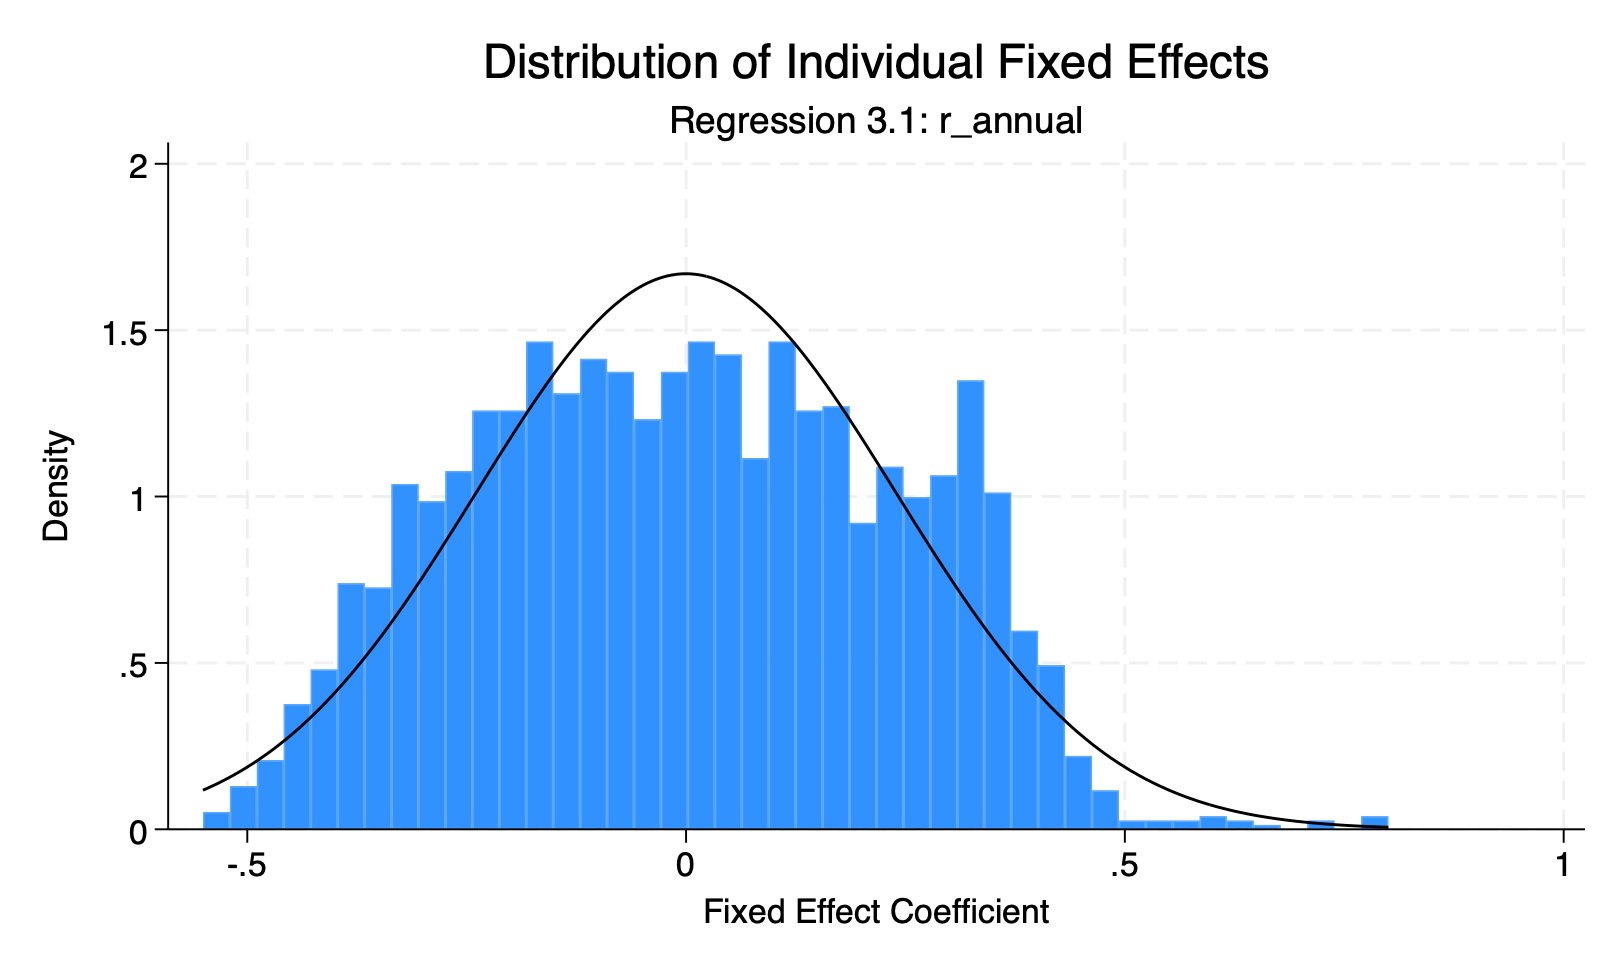
\includegraphics[width=0.8\textwidth]{../Figures/fixed_effects_hist_reg3_1.png}
%\label{fig:PYMPCWealthDecileCompare}
\end{figure}

\begin{figure}[htbp]
\centering
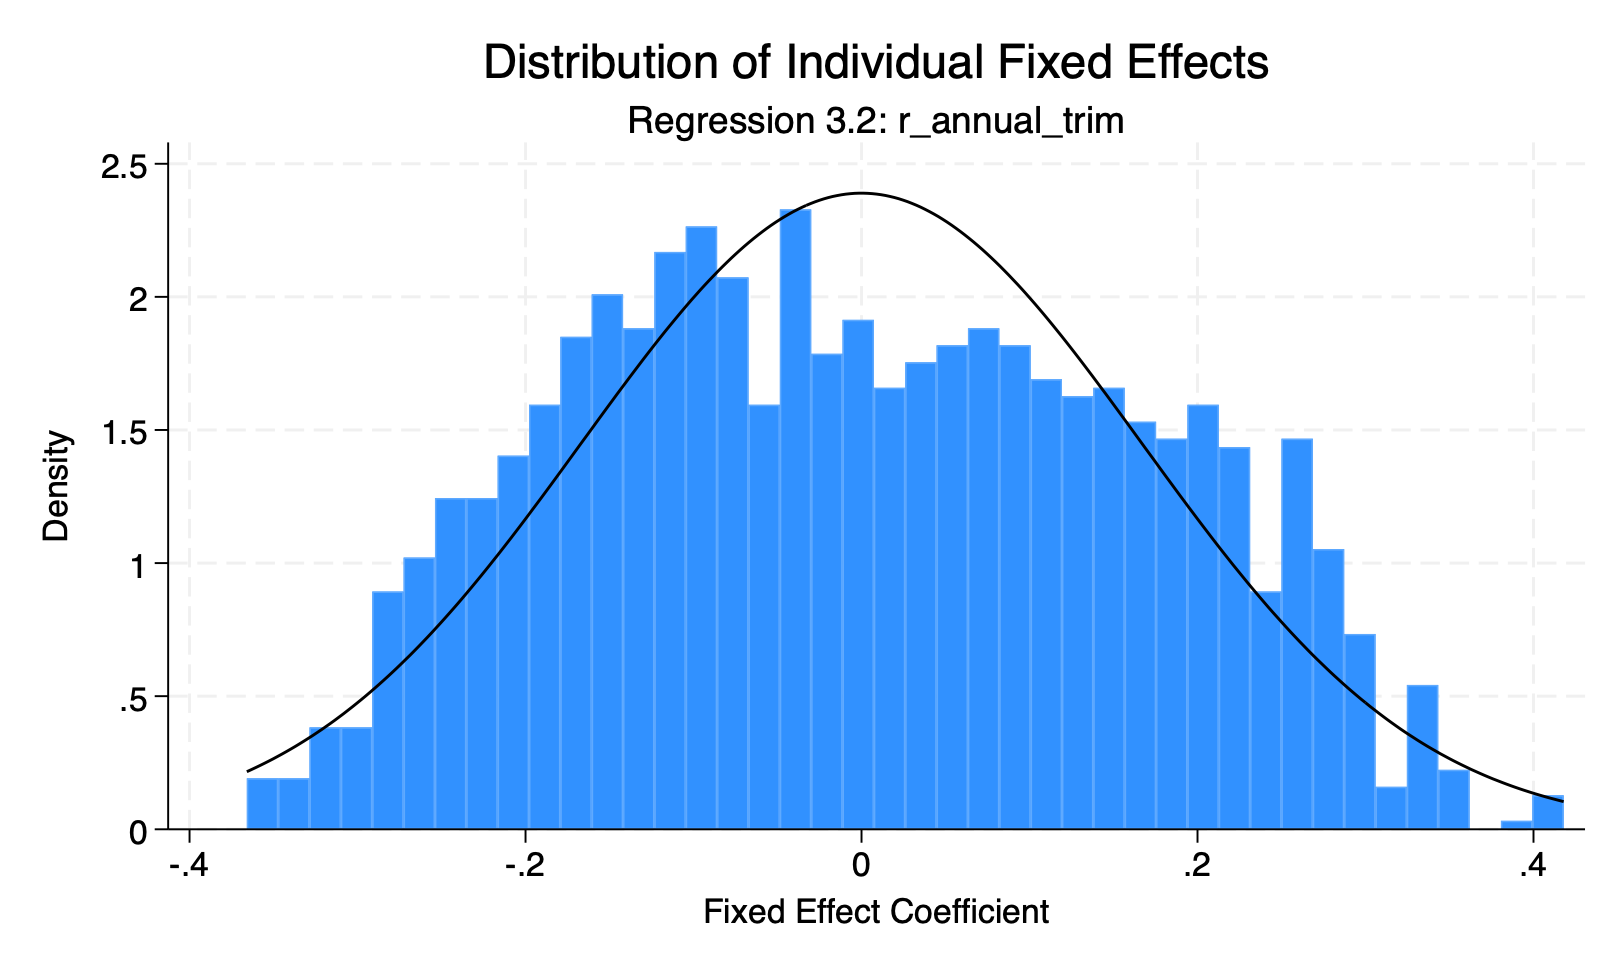
\includegraphics[width=0.8\textwidth]{../Figures/fixed_effects_hist_reg3_2.png}
%\label{fig:PYMPCWealthDecileCompare}
\end{figure}

\begin{figure}[htbp]
\centering
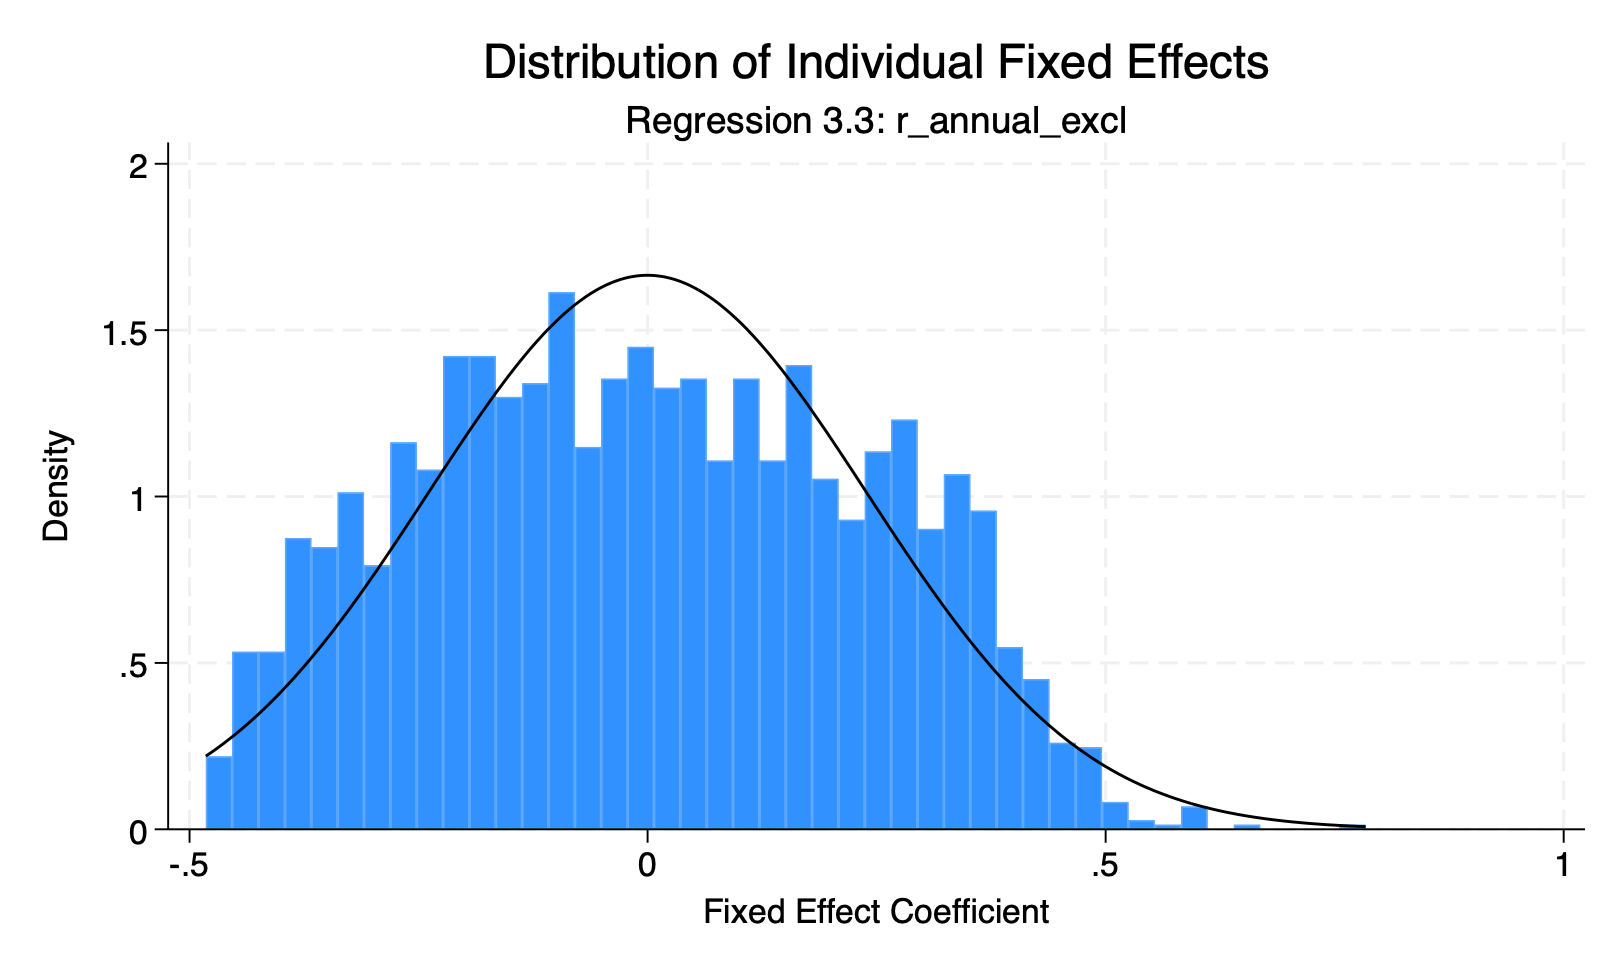
\includegraphics[width=0.8\textwidth]{../Figures/fixed_effects_hist_reg3_3.png}
%\label{fig:PYMPCWealthDecileCompare}
\end{figure}

\begin{figure}[htbp]
\centering
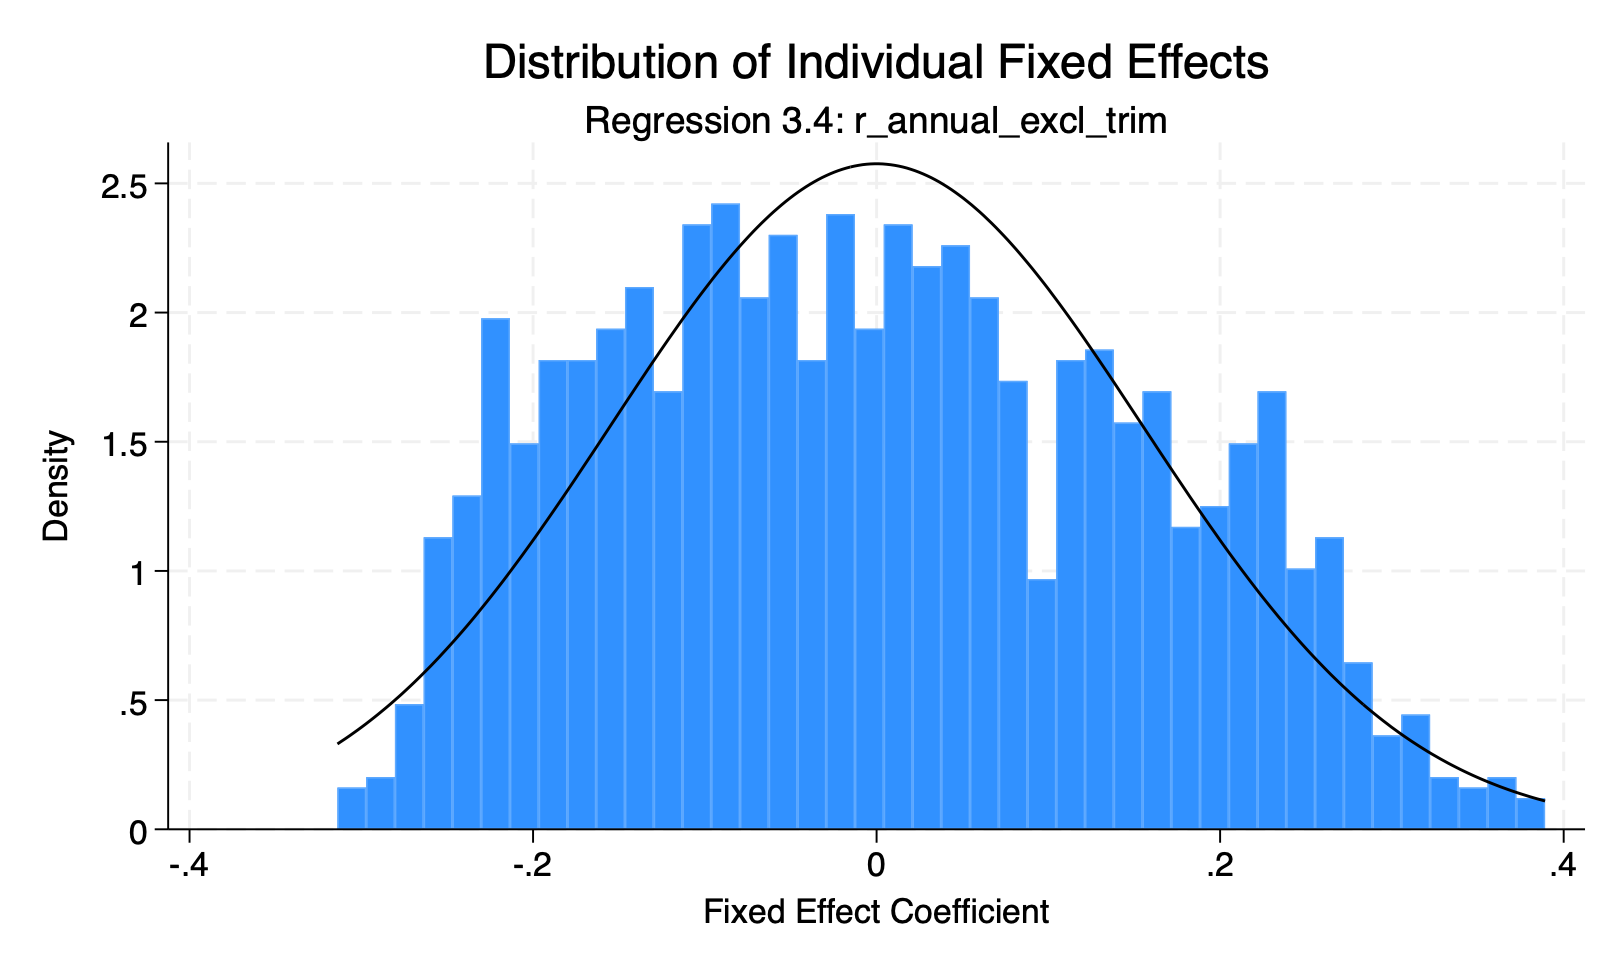
\includegraphics[width=0.8\textwidth]{../Figures/fixed_effects_hist_reg3_4.png}
%\label{fig:PYMPCWealthDecileCompare}
\end{figure}

\subsection{Trust and average returns}

Since the trust module was only conducted in a single survey wave, we have to think of ways to use trust with the panel data. The first is to take the average returns over the 11 waves and use that as the dependen variables. Below are graphs similar to the exercise we did for returns in 2022. The results are not encouraging in this case. 

\begin{landscape}

\begin{table}[htbp]
\centering

% define the star macro
\def\sym#1{\ifmmode^{#1}\else\(^{#1}\)\fi}

\caption{Average Returns (2002–2022) on Trust rv557}

% ---- scale only the tabular ----
\scalebox{0.85}{%
\begin{tabular}{l*{8}{c}}
\toprule
          &\multicolumn{1}{c}{(1)}&\multicolumn{1}{c}{(2)}&\multicolumn{1}{c}{(3)}&\multicolumn{1}{c}{(4)}&\multicolumn{1}{c}{(5)}&\multicolumn{1}{c}{(6)}&\multicolumn{1}{c}{(7)}&\multicolumn{1}{c}{(8)}\\
          &\multicolumn{1}{c}{Avg Annual}&\multicolumn{1}{c}{Avg Annual (trim)}&\multicolumn{1}{c}{Avg Excl. res.}&\multicolumn{1}{c}{Avg Excl. res. (trim)}&\multicolumn{1}{c}{Avg Annual}&\multicolumn{1}{c}{Avg Annual (trim)}&\multicolumn{1}{c}{Avg Excl. res.}&\multicolumn{1}{c}{Avg Excl. res. (trim)}\\
& \multicolumn{4}{c}{No controls} & \multicolumn{4}{c}{With controls} \\\\ 
\cmidrule(lr){2-5}\cmidrule(lr){6-9}
Trust     &    0.021\sym{***}&    0.008         &    0.015\sym{***}&    0.012\sym{***}&    0.012         &    0.004         &    0.006         &    0.006         \\
          &  (0.008)         &  (0.005)         &  (0.005)         &  (0.003)         &  (0.008)         &  (0.005)         &  (0.005)         &  (0.004)         \\
Trust$^{2}$&   -0.002\sym{**} &   -0.001\sym{*}  &   -0.001\sym{**} &   -0.001\sym{***}&   -0.001         &   -0.001         &   -0.001         &   -0.001         \\
          &  (0.001)         &  (0.000)         &  (0.000)         &  (0.000)         &  (0.001)         &  (0.000)         &  (0.000)         &  (0.000)         \\
Age       &                  &                  &                  &                  &    0.010         &    0.017\sym{*}  &    0.014         &    0.020\sym{***}\\
          &                  &                  &                  &                  &  (0.017)         &  (0.010)         &  (0.018)         &  (0.008)         \\
Age$^{2}$ &                  &                  &                  &                  &   -0.000         &   -0.000\sym{*}  &   -0.000         &   -0.000\sym{***}\\
          &                  &                  &                  &                  &  (0.000)         &  (0.000)         &  (0.000)         &  (0.000)         \\
Years of education&                  &                  &                  &                  &    0.003         &    0.002         &    0.004\sym{*}  &    0.002\sym{**} \\
          &                  &                  &                  &                  &  (0.002)         &  (0.001)         &  (0.002)         &  (0.001)         \\
In labor force&                  &                  &                  &                  &    0.025         &   -0.001         &    0.016         &   -0.008         \\
          &                  &                  &                  &                  &  (0.018)         &  (0.014)         &  (0.015)         &  (0.010)         \\
Married   &                  &                  &                  &                  &   -0.010         &   -0.005         &   -0.012         &    0.004         \\
          &                  &                  &                  &                  &  (0.012)         &  (0.009)         &  (0.011)         &  (0.006)         \\
Born in U.S.&                  &                  &                  &                  &   -0.004         &   -0.020\sym{**} &   -0.001         &   -0.014         \\
          &                  &                  &                  &                  &  (0.010)         &  (0.009)         &  (0.016)         &  (0.009)         \\
\_cons    &    0.025         &    0.051\sym{***}&    0.006         &   -0.007         &   -0.264         &   -0.539         &   -0.472         &   -0.740\sym{**} \\
          &  (0.021)         &  (0.013)         &  (0.010)         &  (0.007)         &  (0.646)         &  (0.373)         &  (0.695)         &  (0.286)         \\
\midrule
Observations&  208.000         &  135.000         &  213.000         &  127.000         &  208.000         &  135.000         &  212.000         &  126.000         \\
Adj. R-squared&    0.013         &    0.011         &    0.008         &    0.032         &    0.047         &    0.036         &    0.055         &    0.073         \\
\bottomrule
\multicolumn{9}{l}{\footnotesize Standard errors in parentheses}\\
\multicolumn{9}{l}{\footnotesize Robust SEs in parentheses; Age entered quadratically when available.}\\
\multicolumn{9}{l}{\footnotesize Controls (when included): raedyrs, in labor force, married, born in U.S.}\\
\multicolumn{9}{l}{\footnotesize \sym{*} \(p<0.10\), \sym{**} \(p<0.05\), \sym{***} \(p<0.01\)}\\
\end{tabular}
}% end scalebox
\end{table}


\end{landscape}

\begin{landscape}

  \begin{table}[htbp]
\centering

% define the star macro
\def\sym#1{\ifmmode^{#1}\else\(^{#1}\)\fi}

\caption{Average Returns (2002–2022) on Trust PC1}

% ---- scale only the tabular ----
\scalebox{0.85}{%
\begin{tabular}{l*{8}{c}}
\toprule
          &\multicolumn{1}{c}{(1)}&\multicolumn{1}{c}{(2)}&\multicolumn{1}{c}{(3)}&\multicolumn{1}{c}{(4)}&\multicolumn{1}{c}{(5)}&\multicolumn{1}{c}{(6)}&\multicolumn{1}{c}{(7)}&\multicolumn{1}{c}{(8)}\\
          &\multicolumn{1}{c}{Avg Annual}&\multicolumn{1}{c}{Avg Annual (trim)}&\multicolumn{1}{c}{Avg Excl. res.}&\multicolumn{1}{c}{Avg Excl. res. (trim)}&\multicolumn{1}{c}{Avg Annual}&\multicolumn{1}{c}{Avg Annual (trim)}&\multicolumn{1}{c}{Avg Excl. res.}&\multicolumn{1}{c}{Avg Excl. res. (trim)}\\
& \multicolumn{4}{c}{No controls} & \multicolumn{4}{c}{With controls} \\\\ 
\cmidrule(lr){2-5}\cmidrule(lr){6-9}
Trust PC1 &    0.006         &   -0.002         &    0.007         &    0.006         &    0.005         &    0.000         &    0.007         &    0.007         \\
          &  (0.006)         &  (0.005)         &  (0.004)         &  (0.004)         &  (0.006)         &  (0.005)         &  (0.004)         &  (0.005)         \\
Trust PC1$^{2}$&   -0.004         &   -0.002         &   -0.005\sym{*}  &    0.001         &   -0.001         &   -0.001         &   -0.002         &    0.001         \\
          &  (0.004)         &  (0.003)         &  (0.003)         &  (0.004)         &  (0.004)         &  (0.003)         &  (0.003)         &  (0.004)         \\
Age       &                  &                  &                  &                  &    0.020         &    0.024\sym{**} &    0.023         &    0.028\sym{***}\\
          &                  &                  &                  &                  &  (0.018)         &  (0.011)         &  (0.020)         &  (0.009)         \\
Age$^{2}$ &                  &                  &                  &                  &   -0.000         &   -0.000\sym{**} &   -0.000         &   -0.000\sym{***}\\
          &                  &                  &                  &                  &  (0.000)         &  (0.000)         &  (0.000)         &  (0.000)         \\
Years of education&                  &                  &                  &                  &    0.004         &    0.002         &    0.004\sym{*}  &    0.002         \\
          &                  &                  &                  &                  &  (0.002)         &  (0.002)         &  (0.002)         &  (0.001)         \\
In labor force&                  &                  &                  &                  &    0.032\sym{*}  &   -0.001         &    0.018         &   -0.007         \\
          &                  &                  &                  &                  &  (0.019)         &  (0.016)         &  (0.016)         &  (0.010)         \\
Married   &                  &                  &                  &                  &   -0.005         &   -0.005         &   -0.010         &    0.007         \\
          &                  &                  &                  &                  &  (0.013)         &  (0.010)         &  (0.011)         &  (0.007)         \\
Born in U.S.&                  &                  &                  &                  &   -0.009         &   -0.023\sym{*}  &   -0.012         &   -0.020\sym{*}  \\
          &                  &                  &                  &                  &  (0.012)         &  (0.012)         &  (0.018)         &  (0.010)         \\
\_cons    &    0.083\sym{***}&    0.065\sym{***}&    0.047\sym{***}&    0.019\sym{***}&   -0.616         &   -0.777\sym{*}  &   -0.780         &   -1.004\sym{***}\\
          &  (0.007)         &  (0.005)         &  (0.006)         &  (0.004)         &  (0.692)         &  (0.405)         &  (0.750)         &  (0.321)         \\
\midrule
Observations&  185.000         &  116.000         &  190.000         &  109.000         &  185.000         &  116.000         &  189.000         &  108.000         \\
Adj. R-squared&   -0.004         &   -0.013         &    0.005         &    0.008         &    0.069         &    0.030         &    0.087         &    0.107         \\
\bottomrule
\multicolumn{9}{l}{\footnotesize Standard errors in parentheses}\\
\multicolumn{9}{l}{\footnotesize Robust SEs in parentheses; Age entered quadratically when available.}\\
\multicolumn{9}{l}{\footnotesize Controls (when included): raedyrs, in labor force, married, born in U.S.}\\
\multicolumn{9}{l}{\footnotesize PC1 variance prop =      .}\\
\multicolumn{9}{l}{\footnotesize \sym{*} \(p<0.10\), \sym{**} \(p<0.05\), \sym{***} \(p<0.01\)}\\
\end{tabular}
}% end scalebox
\end{table}



\end{landscape}